%%%%%%%%%%%%%%%%%%%%%%%%%%%%%%%%%%%%%%%%%%%%%%%%%%%%%%%%%%%%%%%%%%%%%%%%%%%
%%
%%  title.tex
%%
%%  Created: Fri Oct 10 14:43:04 1997
%%  Author.: Jose Carlos Gonzales
%%  Notes..:
%%          
%%-------------------------------------------------------------------------
%% Filename: $RCSfile$
%% Revision: $Revision$
%% Date:     $Date$
%%%%%%%%%%%%%%%%%%%%%%%%%%%%%%%%%%%%%%%%%%%%%%%%%%%%%%%%%%%%%%%%%%%%%%%%%%%
%

%%\def\mititulo{%
%%Simulation of \\%
%%Very High Energy \\%
%%Atmospheric Showers\\%
%%for The MAGIC Telescope\\}

%\def\mititulo{%
%Simulation of \\%
%Atmospheric Showers\\%
%and Performance Studies\\%
%for Cherenkov Telescopes\\}

\def\mititulo{%
Simulation and \\%
Performance Studies\\%
for Imaging Cherenkov Telescopes\\%
using Monte Carlo Techniques\\}

\def\mititulogrande{%
Simulation and \\%
Performance Studies\\%
for Imaging Cherenkov\\%
Telescopes using\\%
Monte Carlo Techniques\\}

\def\yo{Jos{\'{e}} Carlos Gonz{\'{a}}lez Garc{\'{\i}}a-Consuegra}

%%============================================================

\thispagestyle{empty}  

\mbox{} \vskip 30pt

\begin{center}
  {\fontsize{30}{35}\selectfont \scshape \mititulogrande}
  \vskip 50pt
  {\centering 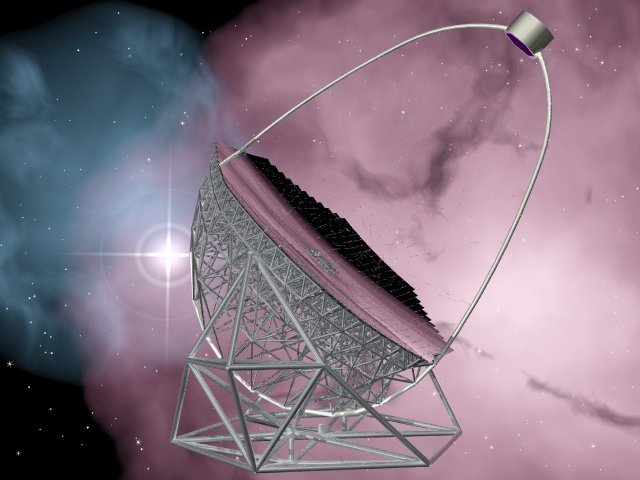
\includegraphics[width=8.5cm]{realmagic1}}
  \vskip 50pt
  {\huge \yo}
  \vskip 50pt
  {\LARGE Septiembre, 2\,000 \\} 
\end{center}

\echapter %%==================================================

\thispagestyle{empty}  

\mbox{} \vskip 50pt

\begin{center}
  {\Huge \sffamily \bfseries \sc \mititulo}
  \vskip 80pt
  {\large \itshape
    Memoria presentada por  \vskip 25 pt
    {\Large \bfseries \rm \yo}  \vskip 25 pt
    para optar al grado de Doctor en Ciencias F{\'{\i}}sicas. \vskip 40pt
    Dirigida por la profesora \vskip 25pt
    {\Large \bfseries \rm Dra. Mar{\'{\i}}a Victoria Fonseca Gonz{\'{a}}lez}
    } \vskip 45pt
  {\Large \rm Septiembre, 2\,000 \\} \vskip 45pt
  
  {\it \small
    Depto. de F{\'{\i}}sica At{\'{o}}mica, Molecular y Nuclear\\
    Facultad de Ciencias F{\'{\i}}sicas\\
    Universidad Complutense de Madrid\\
    }  
\end{center}

\echapter %%==================================================

\thispagestyle{empty}  

\vspace*{2cm}
\begin{flushright}
  \rule{.7\linewidth}{1pt}\\
  \Large \mititulo
  \rule{.7\linewidth}{1pt}
\end{flushright}
\vspace*{6cm}
\begin{flushright}
  \large 
Jos{\'{e}} Carlos Gonz{\'{a}}lez Garc{\'{\i}}a-Consuegra\\[15 mm]
Depto. F{\'{\i}}sica At{\'{o}}mica, Molecular y Nuclear\\
Facultad de Ciencias F{\'{\i}}sicas\\
Universidad Complutense de Madrid\\[15 mm]
Septiembre, 2\,000
\end{flushright}

\echapter %%==================================================

\thispagestyle{empty}  

\vspace*{2cm} 
%
\hfill 
\parbox[b]{0.65\linewidth}{ 
%
\itshape
%
\raggedright
%
There is a theory which states that if ever anyone discovers exactly
what the Universe is for and why it is here, it will instantly
disappear and be replaced by something even more bizarre and
inexplicable. \\
%
\vspace{5pt}
\centerline{---}
\vspace{5pt}
%
There is another theory which states that this has already happened. \\
%
\vspace{15pt}
%
\upshape
%
\raggedleft
%
{\footnotesize (Douglas Adams, ``The Restaurant at the End of the
  Universe'')}
%
} 

\echapter %%==================================================

\endinput
%
%% Local Variables:
%% mode:latex
%% TeX-master: t
%% End:

%%EOF
